\documentclass[a4paper,10pt,notitlepage,pdftex,headsepline]{scrartcl}

\usepackage{geometry}
\geometry{left=2cm}

\usepackage{cmap} % чтобы работал поиск по PDF
\usepackage[utf8]{inputenc}
\usepackage[ukrainian]{babel}
\usepackage[T2A]{fontenc}

\usepackage{textcase}
\usepackage[pdftex]{graphicx}

\pdfcompresslevel=9 % сжимать PDF
\usepackage{pdflscape} % для возможности альбомного размещения некоторых страниц
\usepackage[pdftex]{hyperref}
% настройка ссылок в оглавлении для pdf формата
\hypersetup{unicode=true,
    pdftitle={Курсовая ргр по ТеорПрог},
    pdfauthor={Погода Михаил, Превир Николай},
%    pdfcreator={pdflatex},
    pdfsubject={Визуализация красно-чёрного дерева},
%    pdfborder    = {0 0 0},
%    bookmarksopen,
    bookmarksnumbered,
    bookmarksopenlevel = 2,
    pdfkeywords={Расчётно-графическая работа},
    colorlinks=true, % установка цвета ссылок в оглавлении
    citecolor=black, 
    filecolor=black,
    linkcolor=black,
    urlcolor=blue
}

\usepackage{moreverb}
\author{Michael Pogoda \and Mykola Previr}
\title{ThPrL3}
\date{22.02.2011}

\begin{document}
\thispagestyle{empty}
\begin{center}
\textbf{\Large
\MakeUppercase{Міністерство освіти й науки України}\\
\MakeUppercase{Національний технічний університет України}\\
\MakeUppercase{,,Київський політехнічний інститут''}\\
}

\vspace{2cm}

\textbf{\large
Факультет прикладної математики
}\\

\vspace{3cm}

Курсова розрахунково-графічна робота\\

з дисципліни ,,теорія програмування''

\textbf{Варіант 10 (30 балів)}

\textbf{Візуалізація червоно-чорного дерева}
\end{center}

Виконали:\\
Студент групи\hfill\texttt{КМ-92}\hspace{1cm}\textit{Погода Михайло Володимирович}\hspace{3.5cm}\\
Студент групи\hfill\texttt{КМ-92}\hspace{1cm}\textit{Превір Микола Всеволодович}\hspace{3.5cm}\\

\vspace{1cm}

Перевірив:\\
ПЗ працює\\
Викладач\hfill\textit{Дрозденко О.\,М.}\hfill\underline{\hspace{2cm}}\hspace{0.5cm}\underline{\hspace{2cm}}\\
\texttt{Оцінка}~\underline{\hspace{2cm}}\\
Ст.\,викладач\hfill\textit{Сирота С.\,В.}\hfill\underline{\hspace{2cm}}\hspace{0.5cm}\underline{\hspace{2cm}}

\vfill
\begin{center}

\Large
\bf
КИЇВ 2011

\end{center}

\newpage
\tableofcontents
\newpage
\section{Завдання}
Написати програму, яка реалізує й візуалізує структуру даних і операції над нею згідно вибраного варіанту:

\texttt{Варіант 10.} \textit{Візуалізація червоно-чорного дерева} (5 балів)

Операції:
\begin{itemize}
\item зчитування дерева з лінійної структури;
\item пошук елемента за ключем Fetch(key);
\item вставка елемента згідно ключа Insert(key);
\item видалити елемента за ключем Delete(key);
\item запис дерева в лінійну структуру Dump.
\end{itemize}
\section{Постановка задачі}
Змоделювати й реалізувати структуру даних (клас), що задовольняє вимогам завдання. Програма повинна зображувати червоно-чорне дерево під час роботи алгорітма.
\section{Використані теоретичні відомості}
\begin{itemize}
\item \verb|http://en.wikipedia.org/wiki/Red-black_tree|
\item \verb|http://eternallyconfuzzled.com/tuts/datastructures/jsw_tut_rbtree.aspx|
\end{itemize}
\section{Алгоритм роботи програми}
Клас, що був написаний мною під час виконання даної лабораторної роботи, реалізує червоно-чорне бінарне дерево пошуку.
Візуалізація реалізована за допомоги бібліотеки Graphviz (\url{www.graphviz.org}).
Під час роботи алгорітму дерево малюється кілька разів, з виділеними активними вершинами.
Після цього програма графічного інтерфейсу користувача дозволяє переглядати ці кроки.

\textbf{Червоно-чорне бінарне дерево} --- різновид бінарного дерева пошуку, вершини якого мають додаткові властивості (RB-властивості), зокрема ,,колір'' (червоний або чорний).
Червоно-чорні дерева --- різновид збалансованих дерев, в яких за допомогою спеціальних трансформацій гарантується, що висота дерева $h$ не буде перевищувати $O(\log n)$.
Зважаючи на те, що час виконання основних операцій на бінарних деревах (пошук, видалення, додавання елементу) є $O(h)$, ці структури даних на практиці є набагато ефективнішими, аніж звичайні бінарні дерева пошуку.

Бінарне дерево називається червоно-чорним, якщо воно має такі властивості:
\begin{enumerate}
\item кожна вершина або червона, або чорна;
\item корінь дерева --- чорний;
\item кожний лист (NIL) --- чорний;
\item якщо вершина червона, обидві її дитини чорні;
\item усі шляхи від кореня до листів мають однакову кількість чорних вершин.
\end{enumerate}
Такі властивості надають червоно-чорному дереву додаткового обмеження:
найдовший шлях з кореня до будь-якого листа перевищує найкоротший шлях не більше ніж вдвічі.
В цьому сенсі таке дерево можна назвати збалансованим.
Зважаючи на те, що час виконання основних операцій з бінарними деревами пошуку залежить від висоти, таке обмеження гарантує їхню ефективність в найгіршому випадку, чого звичайні бінарні дерева гарантувати не можуть.

Зазначимо, що в червоно-чорному дереві, відповідно до властивості 4 не існує такого шляху, на якому б зустрілись дві червоні вершини підряд.
Найкоротший шлях складається з усіх чорних вершин, а в найдовшому червоні та чорні вершини чергуються.
З врахуванням властивості 5, отримуємо, що \texttt{глибина будь-яких двох листів відрізняється не більше ніж в два рази}.

В деяких зображеннях червоно-чорних дерев, NIL-листки не наводяться, тому що вони не містять корисної інформації, але їхнє існування необхідне для забезпечення усіх властивостей.

\subsection{Основні операції}
Операції, які не пов'язані з модифікацією RB-дерева, не потребують коректив і повністю аналогічні відповідним операціям для звичайних бінарних дерев пошуку.
Разом з тим, додавання або видалення елементу з червоно-чорного дерева може призвести до порушення RB-властивостей.
Відновлення цих властивостей після модифікації дерева потребує порівняно невеликої кількості ($O(log n)$) операцій зі зміни кольору вершин та не більше як трьох операцій повороту (дві при доданні елементу).
Це залишає часові параметри операцій додавання та видалення в межах $O(log n)$, але ускладнює відповідні алгоритми.

\subsubsection{Вставка елементу}
Процедура починається аналогічно вставці елементу в бінарне дерево пошуку та фарбування її у червоний колір.
Подальші дії залежать від кольорів сусідніх вершин.
Зазначимо, що:
\begin{itemize}
\item властивість 2 завжди зберігається;
\item властивість 3 порушується тільки при вставці червоної вершини, перефарбуванні чорної вершини в червону або обертанні;
\item властивість 4 порушується тільки при вставці чорної вершини, перефарбуванні червоної вершини в чорну або обертанні.
\end{itemize}

Розглянемо такі випадки:
\begin{enumerate}
\item \textit{Нова вершина знаходиться в корені дерева.}
В такому випадку необхідно пофарбувати її в чорний колір для забезпечення властивості 1.
Очевидно, що властивість 5 при цьому залишається справедливою.
\item \textit{Батько нової вершини є чорним.}
Властивість 3 не порушена.
В цьому випадку дерево є коректним.
Властивість 5 також зберігається, адже червона вершина додається на місце чорного листа і це не змінює кількості чорних вершин на цьому шляху.
\item \textit{Батько та дядько доданої вершини є червоними.}
Тоді ми можемо перефарбувати їх обох в чорний, а також перефарбувати дідуся в червоний.
Тепер наша червона вершина має чорного батька.
Завдяки тому, що будь-який шлях через батька чи дядька повинен проходити і через дідуся, кількість чорних вершин на шляху залишається незмінною.
Однак батько дідуся (тобто прадідусь) може бути червоною вершиною, як тепер і дідусь.
Якщо це так, слід повторити цю операцію рекурсивно.
\item[Зауваження] В наступних випадках ми припускаємо, вершина є лівою дитиною. Якщо вона --- права дитина, ліво та право в аналізі наступних випадків слід поміняти місцями.
\item \textit{Батько є червоним, але дядько --- чорний.
До того ж, нова вершина --- права дитина свого батька, і батько в свою чергу ліва дитина свого батька.}
В такому випадку, ми можемо провести лівий поворот, внаслідок якого нова вершина та її батько поміняються ролями.
Подальші дії з минулим батьком проводяться відповідно до випадку 5.
Зважаючи на те, що нова вершина та її батько є червоними, операція повороту не змінює умови 4.
\item \textit{Батько є червоним, але дядько --- чорний.
До того ж, нова вершина -- ліва дитина свого батька, і батько є лівою дитиною свого батька.}
В такому випадку ми проводимо правий поворот навколо дідуся.
В результаті минулий батько тепер є батьком і нової вершини, і свого минулого дідуся.
Ми знаємо, що минулий дідусь є чорним, інакше б батько не був червоним.
Тепер слід поміняти місцями кольори минулого батька та дідуся, і тепер дерево виконує властивість 3.
Легко бачити, що властивість 4 також залишається незмінною.
\end{enumerate}
\subsubsection{Видалення елементу}
Під час видалення вершини можна провести аналогічні міркування й отримати схожий алгоритм (але більш складний).
Під час видалення вершини потрібно не більш ніж три повороти.
\section{Опис програми (інструкції користувача)}
Користувач може змінити інтерфейсні методи класів відповідно до своїх потреб.
За замовчанням, як хеш-функція використовується стандартний метод \verb|.hash| мови програмування Ruby.

\subsection{Опис програми-прикладу}
Програма-приклад є діалогом, що дозволяє виконувати усі можливі дії над змодельованою структурою даних за допомогою графічного інтерфейсу користувача.
Діалогове вікно містить наступні елементи керування(кнопки):
\begin{itemize}
\item \texttt{New} --- створити нове дерево (обнулити поточне);
\item \texttt{Load} --- загрузити дерево з файлу (кожна строчка файлу є вершиною);
\item \texttt{Save} --- зберегти дерево у поточний файл;
\item \texttt{Save as} --- зберегти дерево;
\item \texttt{Add} --- додати введену строку як новий елемент в дерево;
\item \texttt{Remove} --- видалити введений елемент з дерева (за його наявності);
\item \texttt{Search} --- перевірити наявність введеного елемента в дереві;
\item \texttt{Quit} --- вийти з програми.
\end{itemize}
\section{Висновки}
Під час виконання цієї лабораторної роботи була досліджена така інформаційна структура даних, як бінарне дерево пошуку, а саме червоно-чорне дерево.
Ця структура використовується досить часто за рахунок того, що вона відносно нескладно алгоритмізується й, в той же час, має непогані часові характеристики.
\section{Вихідний текст}
\subsection{template\_tree.rb}
\listinginput{1}{ruby.visualization/template_tree.rb}
\subsection{rbtree.rb}
\listinginput{1}{ruby.visualization/rbtree.rb}
\subsection{print\_tree.rb}
\listinginput{1}{ruby.visualization/print_tree.rb}
\subsection{mform.rb}
\listinginput{1}{ruby.visualization/mform.rb}
\subsection{start.rb}
\listinginput{1}{ruby.visualization/start.rb}
\section{Скріншоти}
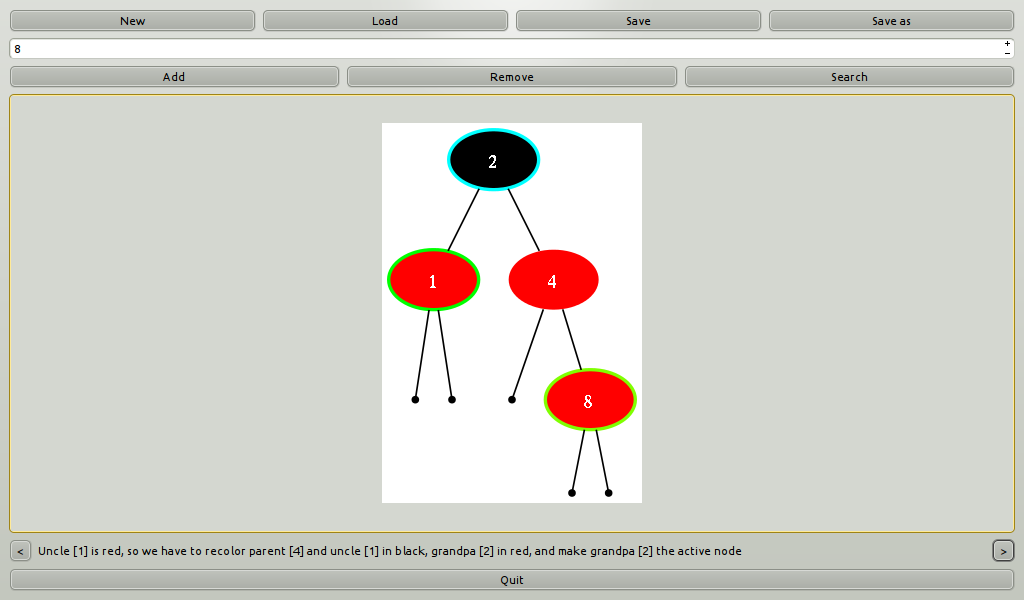
\includegraphics[scale=0.5]{1.png}
\end{document}
